\documentclass[english,a4paper,12pt,oneside]{article}

\usepackage{titlesec}
\titleformat{\section}{\bfseries\Large}{Task \thesection:}{1em}{}

%\includeonly{lab4}

%Drafting options
%uncomment for double spacing
%\doublespacing 

% \usepackage{acronym}
\usepackage{times}
\usepackage{setspace} 
\usepackage{amsmath}    % need for subequations
\usepackage{graphicx}   % need for figures
%\usepackage{picture}
% \usepackage{wrapfig}
\usepackage{graphics}
 \graphicspath{{./}{../Lab-04-Image_statistics/}{../Lab-04-Image_statistics/octave/}{../Lab-04-Image_statistics/data/}}
 \usepackage{epstopdf}
\usepackage{color}
\usepackage{listings}
\lstset{language=C++,
	basicstyle=\ttfamily\footnotesize,
	breaklines=true,
%    basicstyle=\ttfamily,
    keywordstyle=\color{blue}\ttfamily,
    stringstyle=\color{red}\ttfamily,
    commentstyle=\color{green}\ttfamily,
%    morecomment=[l][\color{magenta}]{\#}
}
\usepackage{verbatim}   % useful for program listings
\usepackage{color}      % use if color is used in text
\usepackage{subfigure}  % use for side-by-side figures
\usepackage{varioref}
\usepackage{anysize}
\usepackage{natbib}
\usepackage{fancyhdr}
% \usepackage{units}
\usepackage{longtable}
%\usepackage{bbding}
%\usepackage{aeguill}
\usepackage[hyphens]{url}
\usepackage{hyperref}

\setlength{\parskip}{8pt plus 2pt minus 2pt}
\setlength{\parindent}{0pt}

\marginsize{2cm}{2cm}{2cm}{2cm}
\fancypagestyle{plain}{%
  \fancyhf{}%
  \renewcommand{\headrulewidth}{0pt}%
  \renewcommand{\footrulewidth}{0pt}%
}

\pagestyle{fancy}
%\renewcommand{\sectionmark}[1]{\markright{\thesection.\ #1}}

\renewcommand{\sectionmark}[1]{\markright{#1}{}}
\renewcommand{\subsectionmark}[1]{\markright{#1}{}}
\renewcommand{\subsubsectionmark}[1]{\markright{#1}{}}

%\renewcommand{\quote}[1]{\textit{\begin{quote}#1\end{quote}}}
\newcommand{\bold}[1]{\emph{\textbf{#1}}}

\newcommand{\varentry}[1]{{\guillemotleft}\emph{#1}{\guillemotright}}
\newcommand{\code}[1]{{\tt #1}}

\headheight 10mm


\rhead{Semester 1}
\chead{}
\lhead{ICP3038 --- Computer Vision}
\rfoot{}
\cfoot{- \thepage  \,\,-}
\lfoot{}

\renewcommand{\headrulewidth}{0.4pt}
\renewcommand{\footrulewidth}{0.4pt} 



\begin{document}
% !TEX root = ./ICP3038_Lab_03.tex

\section*{Laboratory 5: Comparing arrays of floating-point numbers}

Most floating-point numbers end up being slightly inaccurate due to rounding errors. 
It means that numbers expected to be equal (e.g. when calculating the same result through different correct methods) often differ, even if very slightly. 
It means that simple equality tests are likely to fail:

\begin{lstlisting}
    float a = 0.15 + 0.15
    float b = 0.1 + 0.2
    if(a == b) // can be false!
    if(a >= b) // can also be false!
\end{lstlisting}

% 
% The solution is to check not whether the numbers are exactly the same, but whether their difference is very small. 
% The error margin that the difference is compared to is often called ``epsilon''. The most simple form:
% 
% \begin{lstlisting}
%     if (abs(a - b) < 0.00001) // wrong - don't do this
% \end{lstlisting}
% 
% This is a bad way to do it because a fixed epsilon chosen because it ``looks small'' could actually be way too large when the numbers being compared are very small as well. 
% In this case the comparison would return \verb+true+ for numbers that are quite different. 
% Also when the numbers are very large, the epsilon could end up being smaller than the smallest rounding error, so that the comparison always returns \verb+false+. 
% Therefore, it is necessary to consider if the relative error is smaller than epsilon:
% 
% \begin{lstlisting}
%     if (abs(a - b) / b < 0.00001) // still not right!
% \end{lstlisting}
% 
% \begin{itemize}
%  \item     When both \verb+a+ and \verb+b+ are zero. \verb+0.0/0.0+ is ``not a number'', which causes an exception on some platforms, or returns false for all comparisons.
%  \item     When only \verb+b+ is zero, the division yields \verb+infinity+, which may also cause an exception, or is greater than epsilon even when a is smaller.
%  \item     It returns false when both \verb+a+ and \verb+b+ are very small but on opposite sides of zero, even when they’re the smallest possible non-zero numbers.
% \end{itemize}
% 



    
    
%This is a typical script that you will be working with at each
%laboratory session. To work with these scripts efficiently, follow the
%guidelines below.
%\begin{enumerate}
%  \item The script is not a step-by-step tutorial. It introduces the
%    problem but it is your task to solve it.
%
%  \item If you get stuck, make sure that you read \emph{Help} section
%    at the end of the document.
%
%  \item If you still have problems, ask the lecturer, demonstrator or
%    fellow students for help.
%
%  \item Try to do as much work as possible in the class, where it is
%    easier to get help.
%    
%  \item If you need help when working at home, use the Blackboard
%    discussion board.
%    
%  \item Finish all assignments at least a week before the deadline. If you get
%    stuck, you will still have one week to ask for help.
%\end{enumerate}
Our 1-D arrays today, or 2-D images in the assignments, store values as floating-point numbers. 
The aims of today's lab are to compare two arrays of floating-point numbers using:
% \begin{itemize}
%	\item Compute the histogram (with the number of bins as a parameter of the function);
	\begin{itemize}
        \item \verb+operator==+ and \verb+operator!=+ (you'll have to overwrite one of them).
        \item Sum of Absolute Errors (SAE), 
        \item Mean Absolute Errors (MAE), 
		\item Sum of Squared Errors (SSE),
		\item Mean Squared Errors (MSE),
		\item Root Mean Squared Errors (RMSE),  and 
		\item Zero Mean Normalised Cross-Correlation (ZNCC).
    \end{itemize}
% \end{itemize}

Note, today you are working on 1-D arrays. In the 2\textsuperscript{nd} assignment, you'll have to do the same but on 2-D images. 
% These notions will be used in Semester~2 on Computer Vision (CV). 


\section{Where is the code?}

We are going to use the same source code as Lab 4. 
We'll rely on your implementation of 


%Same as usual, we will use CMake to make our lives easier. 
%In the lecture, you saw yesterday that it can be extremely complicated to use the IDE to maintain the project files, etc. particularly if students use Windows, Mac, or Linux. 
%There is a ZIP file on Blackboard with 4 (almost) empty C++ source files. There is also a `CMakeLists.txt' file. 
%It is a good practice to organise your source code using directories, etc. Do not compile code in the same directory as your source code. It can get messy... 
%Extract the ZIP file, and set up the compilation environment using \verb+cmake+. 
%In the GUI, the source directory corresponds to the direction in which `CMakeLists.txt' is. 
%The binary directory is where the code will be compiled. Often, we call this directory `bin'. 
%Once the paths are set, press `Configure'. 
%The first time you run the configuration tool, you have to select a generator.
%If you want to use MSVC++ in the lab, make sure to use \emph{Visual Studio 14 2015 Win64}. 
%For Mac OS X, you may want to use the Xcode generator. 
%For Linux, you may choose Makefile. 
%Once the configuration step is over, press `Generate'. 
%The project files are now ready in the `bin' directory. 
%You can compile the code using the preferred IDE.

% \section{Min/Max/Sum/Average/Variance/Standard deviation}
% 
% You have been given a ZIP file containing a small (incomplete class). 
% For this task, you mostly have to modify \verb+MyVector.cpp+.
% The methods you need to complete are:
\begin{enumerate}
 \item \verb+float getMinValue() const+ (see \verb+std::min_element+ previous labs)
 \item \verb+float getMaxValue() const+ (see \verb+std::max_element+ previous labs)
 \item \verb+float getSum() const+ (see \verb+std::accumulate+ previous labs)
 \item \verb+float getAverage() const+
 \item \verb+float getVariance() const+
 \item \verb+float getStandardDeviation() const+
\end{enumerate}


We will use the same ASCII files:
\begin{itemize}
 \item \verb+y.mat+
 \item \verb+y_quadriple.mat+
 \item \verb+y_noise.mat+
 \item \verb+y_negative.mat+
\end{itemize}
that contain the test data you can use to assess your code. 
Figure~\ref{fig:test data} shows the content of the files. 
% You can load each file in independent instances of the class \verb+MyVector+. 
% Table~\ref{tab:test data} provides statistics about the test data from Figure~\ref{fig:test data}. 
% You can use them to compare the results of your computations. 
\begin{figure}[htb]
\centering
\scalebox{0.75}{% Title: glps_renderer figure
% Creator: GL2PS 1.3.8, (C) 1999-2012 C. Geuzaine
% For: Octave
% CreationDate: Mon Nov 16 16:43:05 2015
\setlength{\unitlength}{1pt}
\begin{picture}(0,0)
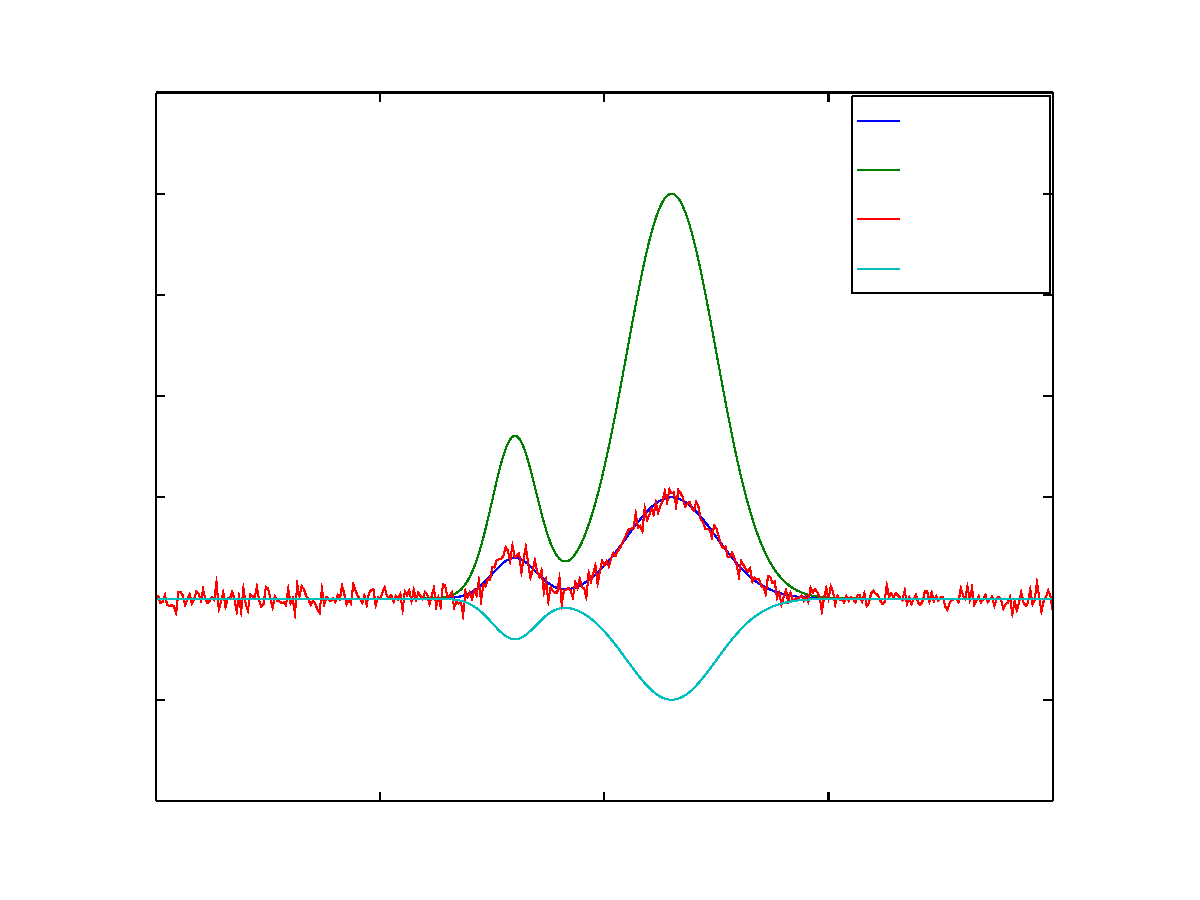
\includegraphics{curves-inc}
\end{picture}%
\begin{picture}(576,432)(0,0)
\fontsize{12}{0}
\selectfont\put(74.8799,42.519){\makebox(0,0)[t]{\textcolor[rgb]{0,0,0}{{-10}}}}
\fontsize{12}{0}
\selectfont\put(182.48,42.519){\makebox(0,0)[t]{\textcolor[rgb]{0,0,0}{{-5}}}}
\fontsize{12}{0}
\selectfont\put(290.08,42.519){\makebox(0,0)[t]{\textcolor[rgb]{0,0,0}{{0}}}}
\fontsize{12}{0}
\selectfont\put(397.68,42.519){\makebox(0,0)[t]{\textcolor[rgb]{0,0,0}{{5}}}}
\fontsize{12}{0}
\selectfont\put(505.28,42.519){\makebox(0,0)[t]{\textcolor[rgb]{0,0,0}{{10}}}}
\fontsize{12}{0}
\selectfont\put(69.8755,47.52){\makebox(0,0)[r]{\textcolor[rgb]{0,0,0}{{-10}}}}
\fontsize{12}{0}
\selectfont\put(69.8755,96.103){\makebox(0,0)[r]{\textcolor[rgb]{0,0,0}{{-5}}}}
\fontsize{12}{0}
\selectfont\put(69.8755,144.686){\makebox(0,0)[r]{\textcolor[rgb]{0,0,0}{{0}}}}
\fontsize{12}{0}
\selectfont\put(69.8755,193.269){\makebox(0,0)[r]{\textcolor[rgb]{0,0,0}{{5}}}}
\fontsize{12}{0}
\selectfont\put(69.8755,241.852){\makebox(0,0)[r]{\textcolor[rgb]{0,0,0}{{10}}}}
\fontsize{12}{0}
\selectfont\put(69.8755,290.434){\makebox(0,0)[r]{\textcolor[rgb]{0,0,0}{{15}}}}
\fontsize{12}{0}
\selectfont\put(69.8755,339.017){\makebox(0,0)[r]{\textcolor[rgb]{0,0,0}{{20}}}}
\fontsize{12}{0}
\selectfont\put(69.8755,387.6){\makebox(0,0)[r]{\textcolor[rgb]{0,0,0}{{25}}}}
\fontsize{12}{0}
\selectfont\put(290.08,397.6){\makebox(0,0)[b]{\textcolor[rgb]{0,0,0}{{Test data}}}}
\fontsize{12}{0}
\selectfont\put(434.47,374.002){\makebox(0,0)[l]{\textcolor[rgb]{0,0,0}{{$Y$}}}}
\fontsize{12}{0}
\selectfont\put(434.47,350.337){\makebox(0,0)[l]{\textcolor[rgb]{0,0,0}{{$Y_{quadriple}$}}}}
\fontsize{12}{0}
\selectfont\put(434.47,326.672){\makebox(0,0)[l]{\textcolor[rgb]{0,0,0}{{$Y_{noise}$}}}}
\fontsize{12}{0}
\selectfont\put(434.47,303.008){\makebox(0,0)[l]{\textcolor[rgb]{0,0,0}{{$Y_{negative}$}}}}
\end{picture}
}
 \caption{\label{fig:test data}Test data from the ASCII files.}
\end{figure}
% \begin{table}[htb]
% \caption{\label{tab:test data}Statistics about the test data from Figure~\ref{fig:test data}}
% \centering
% \begin{footnotesize}
%  \begin{tabular}{|c|c|c|c|c|c|c|}
%   \hline
%   \textbf{Test case} & \textbf{Min} & \textbf{Max} & \textbf{Sum} & \textbf{Average} ($\overline{\mathbf{X}}$)& \textbf{Variance} ($\sigma^2$) & \textbf{Standard deviation} ($\sigma$)\\
%   \hline
%   \hline
%   $\mathbf{Y}$ & 9.5774e-29 & 5 & 300.795 & 0.750113 & 1.8325 & 1.3537 \\
%   \hline
%   $\mathbf{Y_{quadriple}}$ & 3.83096e-28 & 20 & 1203.18 & 3.00045 & 29.3201 & 5.4148 \\
%   \hline
%   $\mathbf{Y_{noise}}$ & -0.837137 & 5.39592 & 303.319 & 0.756407 & 1.94837 & 1.39584 \\
%   \hline
%   $\mathbf{Y_{negative}}$ & -5 & -9.5774e-29 & -300.795 & -0.750113 & 1.8325 & 1.3537 \\
%   \hline
%  \end{tabular}
% \end{footnotesize}
% \end{table}
% 
% Equations~\ref{eq:average} to~\ref{eq:std dev} show how to compute the average, variance and standard deviation of a vector $\mathbf{X}$ of $N$ elements:
% \begin{equation}
%  Average(\mathbf{X}) = \overline{\mathbf{X}} = \frac{1}{N}\sum_{i=0}^{i < N} \mathbf{X}(i)
%  \label{eq:average}
% \end{equation}
% 
% \begin{equation}
%  Variance(\mathbf{X}) = \sigma^2_X = \frac{1}{N}\sum_{i=0}^{i < N}\left(\mathbf{X}(i) - \overline{\mathbf{X}}\right)^2
% \end{equation}
% 
% \begin{equation}
%  Standard\,deviation(\mathbf{X}) = \sigma_X = \sqrt{Variance(\mathbf{X})}
%  \label{eq:std dev}
% \end{equation}



% 





% 
% 
% 
% $$
% 	N = 10 \times \mathrm{randd()}
% $$
% You can use the method \verb+erase+ or \verb+pop_back+. 
% Now, display the smallest and largest values contained in the vector. To do so, use \verb+std::min_element+ and \verb+std::max_element+ provided in the \verb+<algorithm>+ header. Note that these functions return an iterator. Iterators are a bit like pointers. To display the value pointed by an iterator, add a \verb+*+ before it, e.g. \verb+*ite+.
% Finally, display the average value. 
% To get the number of elements in the vector, use its \verb+size()+ method. 
% To get the sum of all the elements of the vector, use \verb+std::accumulate()+ function. 
% It is provided by the \verb+<numeric>+ header. 
% The last parameter is:
% \verb+0+ if you are summing integer numbers,
% \verb+0.0+ for double-precision floating-point numbers, or 
% \verb+0.0f+ for single-precision floating-point numbers.


\section{Task 2: Numerical inaccuracy}

% You may have seen some discrepancies between the values of Table~\ref{tab:test data} and the ones you computed. 
% The differences should be extremely small. 
% The reason is called \emph{numerical inaccuracy}. 
Create a new test program \verb+numerical_inaccuracy.cpp+. 
You need to add it to your \verb+CMakeLists.txt+. 
You need the headers as follows:
\begin{itemize}
\item \verb+iostream+ for printing text in the standard output;
\item \verb+iomanip+ to control how many digits are printed after the dot;
\item \verb+cmath+ to use some mathematical functions.
\end{itemize}
Create 5~single-precision floating-point numbers (32~bit) \verb+i+, \verb+j+, \verb+k+, \verb+l+, and \verb+m+ so that:
\begin{itemize}
	\item \verb+i+ = 10.1111;
	\item \verb+j+ = 20.2222;
	\item \verb+k+ = i + j;
	\item \verb+l+ = j + i; and
	\item \verb+m+ = 30.3333.
\end{itemize}
One would expect \verb+k+, \verb+l+ and \verb+m+ to be equal to~30.3333. 
Print the value in the console with:
\begin{lstlisting}
    std::cout << "k=" << k << "\tl=" << l << "\tm=" << m << std::endl;
\end{lstlisting}
It seems to be the case. 
Let us check this with:
\begin{lstlisting}
    std::cout << k << " is " << (k == l?"the SAME as ":"DIFFERENT from ") << l << std::endl;
    std::cout << k << " is " << (k == m?"the SAME as ":"DIFFERENT from ") << m << std::endl;
    std::cout << l << " is " << (l == m?"the SAME as ":"DIFFERENT from ") << m << std::endl;
\end{lstlisting}

The output I get is as follows:
\begin{verbatim}
k=30.3333  l=30.3333   m=30.3333
30.3333 is the SAME as 30.3333
30.3333 is DIFFERENT from 30.3333
30.3333 is DIFFERENT from 30.3333
\end{verbatim}

As expected \verb+k+ is equal to \verb+l+. 
However, \verb+m+ is not equal to \verb+k+ and \verb+m+ is not equal to \verb+l+. 
In other words, \verb+30.3333+ is not equal to \verb+30.3333+ and \verb+30.3333+ is not equal to \verb+30.3333+. 

\begin{center}{\bf What is going on???}\end{center}

Let us add more zeros after the dot with:
\begin{lstlisting}
   std::cout << std::setprecision(17) << k << "\t" <<
       std::setprecision(17) << l << "\t" <<
       std::setprecision(17) << m << std::endl;
\end{lstlisting}

\verb+k+ and \verb+l+ are equal to 30.333301544189453 but \verb+m+ is equal to 30.33329963684082. 
This is due to what is called numerical inaccuracy. 
At a rule of thumb, {\bf\large DO NOT USE \verb+==+ and \verb+!=+ with floating-point numbers} (\verb+float+ or \verb+double+). 

\begin{center}{\bf What should we do then???}\end{center}


\subsection*{Absolute difference}


The solution is to check not whether the numbers are exactly the same, but whether their difference is very small. 
The error margin that the difference is compared to is often called ``epsilon''. The most simple form is called absolute difference:

\begin{lstlisting}
    if (abs(a - b) < 0.00001) // wrong - don't do this
\end{lstlisting}

This is a bad way to do it because a fixed epsilon chosen because it ``looks small'' could actually be way too large when the numbers being compared are very small as well. 
In this case the comparison would return \verb+true+ for numbers that are quite different. 

Create a new function:
\begin{lstlisting}
    bool isEqual(double a, double b, double epsilon = 0.00001)
    {
        // Check equality using absolute difference
        return (abs(a - b) < epsilon);
    }
\end{lstlisting}
and replace \verb+==+ in your code with the corresponding calls of \verb+isEqual+. 
If the absolute difference is smaller than a threshold \verb+epsilon+ then consider that the two numbers are equal. 
If not, they are different. 
Test your new program. 
It seems better, but...


\subsection*{Relative difference}

when the numbers are very large, the epsilon could end up being smaller than the smallest rounding error, so that the comparison always returns \verb+false+. 
Therefore, it is necessary to consider if the relative error is smaller than epsilon:

\begin{lstlisting}
    if (abs(a - b) / b < epsilon) // still not right!
\end{lstlisting}

We should replace our function with:

\begin{lstlisting}
    bool isEqual(double a, double b, double epsilon = 0.00001)
    {
        // Check equality using absolute difference
        //return (abs(a - b) < epsilon);

        // Check equality using relative difference
        return ((abs(a - b) / b) < epsilon);
    }
\end{lstlisting}


But...
\begin{itemize}
 \item     when both \verb+a+ and \verb+b+ are zero. \verb+0.0/0.0+ is ``not a number'', which causes an exception on some platforms, or returns false for all comparisons.
 \item     when only \verb+b+ is zero, the division yields \verb+infinity+, which may also cause an exception, or is greater than epsilon even when a is smaller.
 \item     it returns false when both \verb+a+ and \verb+b+ are very small but on opposite sides of zero, even when they’re the smallest possible non-zero numbers.
\end{itemize}


\subsection*{Final version of isEqual}

Make sure you include these new headers:
\begin{lstlisting}
#include <climits>
#include <algorithm>
\end{lstlisting}

And replace the function with:

\begin{lstlisting}
    bool isEqual(double a, double b, double epsilon = 0.00001)
    {
        // Check equality using absolute difference
        //return (abs(a - b) < epsilon);

        // Check equality using relative difference
        //return ((abs(a - b) / b) < epsilon);

        // Handle infinities
        if (a == b) return true;
        
        double abs_A    = abs(a);
        double abs_B    = abs(b);
        double abs_diff = abs(a - b);

        // if a or b is zero or both are extremely close to it
        // then relative error is less meaningful
        if (a == 0 || b == 0 || (abs_A + abs_B < std::numeric_limits<float>::min()))
            return abs_diff < std::numeric_limits<float>::min();
        // use relative error
        else
            return ((abs_diff / std::min(abs_A, abs_B)) < epsilon);
    }
\end{lstlisting}





\section{Task 3: operator== and operator!=}

Go back to the \verb+MyVector+ class.
We are going to edit:
\begin{itemize}
\item \verb+ bool MyVector::operator==(const MyVector& aVector) const;+
\item \verb+ bool MyVector::operator!=(const MyVector& aVector) const;+
\end{itemize}

Note that to limit the scope for errors we will reuse the code of \verb+operator==+ in the implementation of \verb+operator!=+:
\begin{lstlisting}
bool MyVector::operator!=(const MyVector& aVector) const
{
	return (!((*this) == aVector));
}
\end{lstlisting}

In our test program, we created:
\begin{lstlisting}
        MyVector temp3(y + y + y + y);
\end{lstlisting}
It should be the same as 4 $\times$ \verb+y+.
However, \verb+temp3 == y_quadriple+ always returns false despite the cout showing the same numerical values. 
It's due to rounding errors.
In the implementation of \verb+operator==+ we MUST use the same technique as what we saw previously in Task~2. 
Add the \verb+isEqual()+ function to \verb+MyVector.cpp+, e.g. at the top of the file. Make sure the header files are included.
In  \verb+ bool MyVector::operator==(const MyVector& aVector) const;+, comment \verb+if (*ite0++ != *ite1++) return (false);+ and use \verb+isEqual()+, e.g.
\begin{lstlisting}
    if (!isEqual(*ite0++, *ite1++)) return (false);
\end{lstlisting}

Re-run your test program.
Now \verb+temp3 == y_quadriple+ returns true.

% To try your new operator, add the code as follows in your test program \verb+test_my_vector.cpp+:
% \begin{lstlisting}
% MyVector temp(y_quadruple / 4.0);
% std::cout << (y == y_quadruple?"SAME":"DIFFERENT") << std::endl;
% \end{lstlisting}

With our new operators, we can check if our 1-D vectors, or 2-D images, are equal or different. We often want to quantify the amount of dissimilarity between two images in computer vision applications. In this case we rely on error (or distance) metrics. An error close to zero means that the two images are similar. The larger the error, the more dissimilar they are.



\section{How dissimilar two vectors are: the SAE}


SAE stands for sum of absolute errors. It is also called sum of absolute distance (SAD), Manhattan distance, and $L^1$-norm.  
In statistics, it is used as a quantity to measure how far two vectors are from each other. 
The SAE between two vectors $\mathbf{Y_1}$ and $\mathbf{Y_2}$ of $N$ element is:
\begin{equation}
SAE(\mathbf{Y_1}, \mathbf{Y_2}) = \sum^{i < N}_{i=0} |\mathbf{Y_1}(i)-\mathbf{Y_2}(i)|
\end{equation}
Add the method as follows in your class:
\begin{lstlisting}
float MyVector::SAE(const MyVector& aVector) const;
\end{lstlisting}

One of the main advantages of the SAE is that it is fast to compute.  
However, it has limitations. 
To test your computations, here are the results for:
\begin{itemize}
\item $SAE(\mathbf{Y}, \mathbf{Y}) =  0$
\item $SAE(\mathbf{Y}, \mathbf{Y_{quadriple}}) =  902.386$
\item $SAE(\mathbf{Y}, \mathbf{Y_{negative}}) =  601.591$
\item $SAE(\mathbf{Y}, \mathbf{Y_{noise}}) =  104.505$
\end{itemize}
$\mathbf{Y_{quadriple}}$ is equal to $4 \times \mathbf{Y}$. 
However, the SAE between $\mathbf{Y_{quadriple}}$ and $\mathbf{Y}$ is the largest. 
$\mathbf{Y_{negative}}$ is equal to $\mathbf{-Y}$. 
However, the SAE between $\mathbf{Y_{negative}}$ and $\mathbf{Y}$ is the second largest. 
We can conclude that even if SAE is commonly used in imaging  it may not provide a good error metrics in some cases.

\section{How dissimilar two vectors are: the MAE}

Sometimes, the Mean Absolute Error (MAE) is used. To get it, just divide the SAE by the number of samples:
\begin{equation}
MAE(\mathbf{Y_1}, \mathbf{Y_2}) = \frac{SAE(\mathbf{Y_1}, \mathbf{Y_2})}{N}
\end{equation}
To test your computations, here are the results for:
\begin{itemize}
\item $MAE(\mathbf{Y}, \mathbf{Y}) =  0$
\item $MAE(\mathbf{Y}, \mathbf{Y_{quadriple}}) =  2.2503$
\item $MAE(\mathbf{Y}, \mathbf{Y_{negative}}) =  1.5002$
\item $MAE(\mathbf{Y}, \mathbf{Y_{noise}}) =  0.26061$
\end{itemize}

\section{How dissimilar two vectors are: the SSE}

SSE stands for sum of squared  errors. It is also called sum of squared distance (SAD), Euclidean distance, and $L^2$-norm.  
\begin{equation}
SSE(\mathbf{Y_1}, \mathbf{Y_2}) = \sum^{i < N}_{i=0} (\mathbf{Y_1}(i)-\mathbf{Y_2}(i))^2
\end{equation}
To test your computations, here are the results for:
\begin{itemize}
\item $SSE(\mathbf{Y}, \mathbf{Y}) =  0$
\item $SSE(\mathbf{Y}, \mathbf{Y_{quadriple}}) =  8644.2$
\item $SSE(\mathbf{Y}, \mathbf{Y_{negative}}) =  3841.9$
\item $SSE(\mathbf{Y}, \mathbf{Y_{noise}}) =  43.341$
\end{itemize}


\section{How dissimilar two vectors are: the MSE}

Sometimes, the Mean Squared Error (MSE) is used. To get it, just divide the SSE by the number of samples:
\begin{equation}
MSE(\mathbf{Y_1}, \mathbf{Y_2}) = \frac{SSE(\mathbf{Y_1}, \mathbf{Y_2})}{N}
\end{equation}
To test your computations, here are the results for:
\begin{itemize}
\item $MSE(\mathbf{Y}, \mathbf{Y}) =  0$
\item $MSE(\mathbf{Y}, \mathbf{Y_{quadriple}}) =  21.557$
\item $MSE(\mathbf{Y}, \mathbf{Y_{negative}}) =  9.5807$
\item $MSE(\mathbf{Y}, \mathbf{Y_{noise}}) =  0.10808$
\end{itemize}

\section{How dissimilar two vectors are: the RMSE}

Sometimes, the Root Mean Squared Error (RMSE) is used. To get it, just return the square root of MSE:
\begin{equation}
RMSE(\mathbf{Y_1}, \mathbf{Y_2}) = \sqrt{MSE(\mathbf{Y_1}, \mathbf{Y_2})}
\end{equation}
To test your computations, here are the results for:
\begin{itemize}
\item $RMSE(\mathbf{Y}, \mathbf{Y}) =  0$
\item $RMSE(\mathbf{Y}, \mathbf{Y_{quadriple}}) =  4.6429$
\item $RMSE(\mathbf{Y}, \mathbf{Y_{negative}}) =  3.0953$
\item $RMSE(\mathbf{Y}, \mathbf{Y_{noise}}) =  0.32876$
\end{itemize}


\section{How similar two vectors are: the ZNCC}

ZNCC stands for Zero Mean Normalised Cross-Correlation. 
The normalisation in ZNCC addresses the limitation highlighted in our tests. 
The formula is:
\begin{equation}
ZNCC(\mathbf{Y_1}, \mathbf{Y_2}) = \frac{1}{N}\sum^{i < N}_{i=0} \frac{(\mathbf{Y_1}(i)-\overline{\mathbf{Y_1}})(\mathbf{Y_2}(i)-\overline{\mathbf{Y_2}})}{\sigma_{Y_1}\sigma_{Y_2}}
\end{equation}
\begin{itemize}
\item $ZNCC(\mathbf{Y_1}, \mathbf{Y_2})$ = 1, if $\mathbf{Y_1}$ and $\mathbf{Y_2}$ are fully correlated (e.g. $\mathbf{Y_1} = \alpha \mathbf{Y_2}$);
\item $ZNCC(\mathbf{Y_1}, \mathbf{Y_2})$ = -1, if $\mathbf{Y_1}$ and $\mathbf{Y_2}$ are fully anti-correlated (e.g. $\mathbf{Y_1} = -\alpha \mathbf{Y_2}$);
\item $ZNCC(\mathbf{Y_1}, \mathbf{Y_2})$ = 0, if $\mathbf{Y_1}$ and $\mathbf{Y_2}$ are fully uncorrelated (they are unrelated).
\end{itemize}
Often the ZNCC is expressed as a percentage. 
With our examples, we get:
\begin{itemize}
\item $ZNCC(\mathbf{Y}, \mathbf{Y}) = 0.999996 =	99.9996\%$
\item $ZNCC(\mathbf{Y}, \mathbf{Y_{quadriple}}) = 0.999996 =	99.9996\%$
\item $ZNCC(\mathbf{Y}, \mathbf{Y_{negative}}) = -0.999996 =	-99.9996\%$
\item $ZNCC(\mathbf{Y}, \mathbf{Y_{noise}}) =  0.97188 =	97.188\%$
\end{itemize}

\section{Error checks}

Have you thought about what to do if the size of the two arrays that you are comparing is different?
If you haven't revisit Tasks~3 to~8 to make sure that the program won't crash.




% 
% \section{Summary and hint for the assignment}
% 
% Today, you saw how to use
% \verb+std::min_element+, \verb+std::max_element+, and \verb+std::accumulate+ to compute some statistical values on vectors. For the assignment, you can adapt your code so that it works for an image store as a 1-D array. Remember, STL iterators behave like pointers: You can use these functions on C arrays:
% 
% \begin{verbatim}
%  int my_array = {-1, 2, 3, 5, 6};
%  int* p_min_element = std::min_element(&my_array[0], &my_array[5]);
%  std::cout << "min = " << *p_min_element << std::endl;
% \end{verbatim}
% 
% \begin{itemize}
%  \item \verb+&my_array[0]+ is the address of the 1st element of the array;
%  \item \verb+&my_array[N-1]+ is the address of the last element of the array (with \verb+N+=5).
%  \item \verb+&my_array[N]+ is the address of the memory cell after the last element of the array.
% \end{itemize}
% 



% 
% 
% compare 1-D vectors in six different ways:
% \begin{itemize}
% \item SAE
% \item MAE
% \item SSE
% \item MSE
% \item RMSE
% \item ZNCC
% \end{itemize}
% You will adapt them to the assignments and use them next Semester to perform computer vision tasks.

%\item $ZNCC_y_y_quadriple =  99.751$
%\item $ZNCC_y_y_negative = -99.751$
%\item $ZNCC_y_y_noise =  96.845$


%
%
%
%
%
%
%For this task, you are given two C++ files:
%\begin{enumerate}
%  \item \verb+include/Utils.h+, a header file with the declarations of some functions.
%  \item \verb+src/TestVector.cpp+, a test program to try the vector class.
%\end{enumerate}
%
%Modify \verb+include/Utils.h+ to convert every function as a template function. 
%To implement every function, you need to write the code directly in the header. 
%In \verb+src/TestVector.cpp+, test every template function with different data types.
%
%
%\section{Task 3: Create your own template class}
%
%This time, you have to create your own files and modify CMakeLists.txt. 
%We propose to create a template class to handle square matrices, e.g. n-by-n matrices. 
%The class should contain:
%\begin{itemize}
%\item a default constructor, 
%\item a copy constructor, 
%\item a copy operator, 
%\item \verb+operator<<+, 
%\item \verb+operator>>+,
%\item \verb+unsigned int m_size+ (default: 4) the number of rows 
%\item \verb+unsigned int getSize() const+
%\item \verb+void setSize(unsigned int)+
%\item \verb+T& get(unsigned int i, unsigned int j) const+
%\item \verb+void set(unsigned int i, unsigned int j, const T& aValue)+
%\item \verb+void setIdentity()+
%\end{itemize}
%Each method should be tested and validated in a test program. 
%Do not wait until the end to test your code. 
%A good programming strategy is to test a function just after it has been implemented. 
\end{document}
